\vspace*{-0.9cm}
\section*{III - Achievements}
\addcontentsline{toc}{section}{III - Achievements}
\subsection*{Orée rouge émerveillant}
\addcontentsline{toc}{subsection}{Orée rouge émerveillant}
\label{sec:ore}
Cet achievement permet de revenir sur les éléments abordés dans la section \hyperref[sec:pos]{\uline{Les positions}}. Il a pour objectif de créer de nouveaux types de plateaux de jeu. Selon une graine donnée, le plateau de jeu pourra avoir des positions invalides ou des cases considérées comme voisines à des positions différentes de celles de base.\\

Ces modifications impacteront les fonctions d'initialisation des positions et de listage des voisins.\\

Dans le cas (1) d'un plateau où les voisins d'une position donnée sont les positions valides accessibles à distance 2, en utilisant uniquement les directions cardinales ou uniquement les directions diagonales, la fonction que nous avions implémentée était adaptable en modifiant simplement la liste des directions à prendre en compte.\\

Dans le cas (2) d'un plateau qui a une géométrie torique, il suffit de faire comme pour un plateau normal mais en ajoutant \texttt{MAX\_X} et \texttt{MAX\_Y} aux coordonnées x et y déterminées, puis en prenant le modulo de ces valeurs pour obtenir les coordonnées sans dépasser les limites du plateau.\\

Dans le cas (3) d'un plateau de jeu "infernal"\footnote{une position sur quatre est invalide}, lors de l'initialisation de la liste des positions, les positions où les coordonnées x ou y sont paires sont initialisées comme invalides. \\ \\
Grâce à notre implémentation précédente, nous avons pu facilement adapter notre code pour ces trois cas en ajoutant simplement des conditions dans les fonctions \texttt{init\_positions} et \texttt{list\_neighbors}.
\subsection*{Messires Roses irrédules}
\addcontentsline{toc}{subsection}{Messires Roses irrédules}
\label{sec:mri}
Jusqu'alors, les mines étaient positionnées aléatoirement sur le plateau de jeu avec un algorithme que nous avions étudié comme peu optimal. Cet achievement a pour objectif de les positionner de manière optimale de la façon suivante~:
\begin{itemize}
    \setlength\itemsep{0.01em}
    \item Calculer le "coût" du placement des mines sur le plateau : la somme des carrés des tailles des amas de mines (un amas est un ensemble de mines adjacentes).
    \item Trouver le placement de mines qui minimise ce coût.
\end{itemize}
\subsubsection*{Calcul du coût}
Le coût est calculé en identifiant les amas de mines sur le plateau de jeu à l'aide d'un algorithme de parcours en profondeur (\textit{Depth-First Search}, DFS)~\cite{cosson2023breadth}.\\
Comme le représente la figure \ref{fig:dfs-example}, la pile est initialisée avec une mine non-visitée et on considère que c'est un nouvel amas.
Tant que la pile est non-vide, on dépile et on incrémente la taille de l'amas, puis on empile les mines voisines non-visitées.
On additionne ensuite le carré de la taille de l'amas au coût.
On répète jusqu'à ce que toutes les mines soient visitées.\\\\
\begin{figure}[!h]
\centering
\resizebox{400px}{!}{
\begin{tikzpicture}
    \draw (0,0) grid (3,3);
\draw[color=red!60, fill=red!5](1,2) rectangle (2,3) node[pos=.5] {1};
    \draw[color=darkgreen!60, fill=darkgreen!5](2,2) rectangle (3,3) node[pos=.5]{2};
    \draw[color=darkgreen!60, fill=darkgreen!5](2,1) rectangle (3,2) node[pos=.5]{3};
    \draw[color=gray!60, fill=gray!5](2,0) rectangle (3,1) node[pos=.5] {4};
    \draw[color=gray!60, fill=gray!5](0,0) rectangle (1,1) node[pos=.5] {5};
    \draw[color=red!60, very thick](0,3) rectangle (3,1);
    \node[draw,align=left] at (1.5,4.5) {pile: [\textcolor{darkgreen}2, \textcolor{darkgreen}{3}] \\ visité: [1,\textcolor{darkgreen}{2},\textcolor{darkgreen}{3}] \\ taille: 3};

    \draw (5,0) grid (8,3);
    \draw[color=blue!60, fill=blue!5](6,2) rectangle (7,3) node[pos=.5] {1};
    \draw[color=red!60, fill=red!5](7,2) rectangle (8,3) node[pos=.5]{2};
    \draw[color=blue!60, fill=blue!5](7,1) rectangle (8,2) node[pos=.5] {3};
    \draw[color=gray!60, fill=gray!5](7,0) rectangle (8,1) node[pos=.5] {4};
    \draw[color=gray!60, fill=gray!5](5,0) rectangle (6,1) node[pos=.5] {5};
    \draw[color=red!60, very thick](6,1) rectangle (8,3);
    \node[draw,align=left] at (6.5,4.5) {pile: [3] \\ visité: [1,2,3] \\ taille: {3}};


    \draw (10,0) grid (13,3);
    \draw[color=blue!60, fill=blue!5](11,2) rectangle (12,3) node[pos=.5] {1};
    \draw[color=blue!60, fill=blue!5](12,2) rectangle (13,3) node[pos=.5]{2};
    \draw[color=red!60, fill=red!5](12,1) rectangle (13,2) node[pos=.5] {3};
    \draw[color=darkgreen!60, fill=darkgreen!5](12,0) rectangle (13,1) node[pos=.5] {4};
    \draw[color=gray!60, fill=gray!5](10,0) rectangle (11,1) node[pos=.5] {5};
    \draw[color=red!60, very thick](11,0) rectangle (13,3);
    \node[draw,align=left] at (11.5,4.5) {pile: [\textcolor{darkgreen}{4}] \\ visité: [1,2,3,\textcolor{darkgreen}{4}] \\ taille: 4};

    \draw (15,0) grid (18,3);
    \draw[color=blue!60, fill=blue!5](16,2) rectangle (17,3) node[pos=.5] {1};
    \draw[color=blue!60, fill=blue!5](17,2) rectangle (18,3) node[pos=.5]{2};
    \draw[color=blue!60, fill=blue!5](17,1) rectangle (18,2) node[pos=.5]{3};
    \draw[color=red!60, fill=red!5](17,0) rectangle (18,1) node[pos=.5] {4};
    \draw[color=gray!60, fill=gray!5](15,0) rectangle (16,1) node[pos=.5] {5};
    \draw[color=red!60, very thick](16,0) rectangle (18,2);
    \node[draw,align=left] at (16.5,4.5) {pile: [] \\ visité: [1,2,3,4] \\ taille: 4};

\end{tikzpicture}
}
\captionof{figure}{Exemple de parcours d'un amas}\label{fig:dfs-example}
\end{figure}
\subsubsection*{Minimisation du coût}
Afin de minimiser le coût, nous avons appliqué une logique intuitive que nous utilisons inconsciemment sur un tableau à une dimension. Comme le montre la figure~\ref{tab:exemple_plateau}, nous avons considéré que pour que les mines soient le plus écartées possible, il faut les positionner toutes les \(\left\lfloor \frac{\texttt{TAB\_SIZE}}{\texttt{NB\_MINE}} \right\rfloor\) cases. Par exemple, pour un tableau de taille 9 avec 3 mines, \(\left\lfloor \frac{9}{3} \right\rfloor = 3\). On place donc une mine toutes les 3 cases.
\begin{center}
\begin{tabular}{|p{0.07\linewidth}|p{0.07\linewidth}|p{0.07\linewidth}|p{0.07\linewidth}|p{0.07\linewidth}|p{0.07\linewidth}|p{0.07\linewidth}|p{0.07\linewidth}|p{0.07\linewidth}|}
\hline
\centering\textbf{\textcolor{green}{\huge $\times$}} & & & \centering\textbf{\textcolor{green}{\huge $\times$}} &  &  & \centering\textbf{\textcolor{green}{\huge $\times$}} &  &\\
\hline
\end{tabular}
\captionof{figure}{Exemple de plateau à une seule dimension}
\label{tab:exemple_plateau}
\end{center}
La position de la première mine est toujours aléatoire afin d'avoir des emplacements de mines différents à chaque partie.\\ \\
Notre plateau étant à deux dimensions, nous avons adapté cette logique pour les deux dimensions:\\
Pour un plateau de \(X \times Y = n\) positions totales avec \(k\) mines à placer, où \(k = \left\lfloor \frac{n}{4} \right\rfloor\). On note \(A = \max(X, Y)\) et \(B = \min(X, Y)\). On devra alors positionner \(k_1 = \left\lfloor\frac{k}{B}\right\rfloor\) mines sur chaque dimension de \(A\) avec une en plus sur les \(r = k\bmod B\) dernières. Elles seront donc espacées de \(dec = \left\lfloor \frac{\max(X, Y)}{k_1} \right\rfloor\) cases. Pour alterner les mines sur la dimension \(B\), dès qu'on a fini de remplir un \(A\), on décale la position de la première mine de \(z = \frac{dec}{2}\) cases.\\
\\ Donc :
\\
1) On considère aléatoirement la position (\(a_{\textsubscript{init}}, b_{\textsubscript{init}}\)). \\
2) Pour \(i\) allant de \(0\) à \(k\), on place les mines aux positions suivantes~:
\begin{itemize}
    \item \(b = b_{\textsubscript{init}} + \left\lfloor \frac{i}{k_1} \right\rfloor \bmod B \)
    \item  \(a =  (a_{\textsubscript{init}} + dec \times i + z \times b)\bmod A\)
    \item Selon si \(A\) est \(X\) ou \(Y\), on place la mine en (\(a, b\)) ou (\(b, a\))
\end{itemize}
La figure~\ref{tab:exemple_plateau_2d} illustre un exemple pour un plateau de taille \(8 \times 5\) avec \(x_{\textsubscript{init}} = 2\) et \(y_{\textsubscript{init}} = 1\).
\begin{center}
    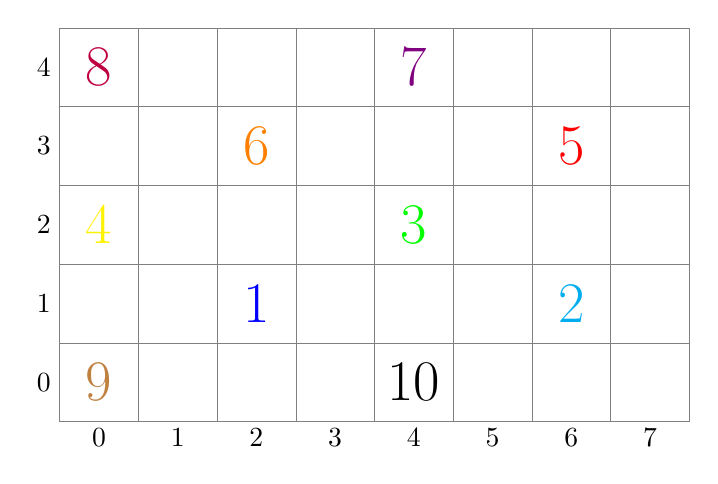
\begin{tikzpicture}
        \draw[step=1cm,gray,very thin] (0,0) grid (8,5);
        \foreach \x in {0,1,...,7} \node at (\x+0.5,-0.2) {\x};
        \foreach \y in {0,1,...,4} \node at (-0.2,\y+0.5) {\y};
        \node at (2.5,1.5) {\textcolor{blue}{\huge 1}};
        \node at (6.5,1.5) {\textcolor{cyan}{\huge 2}};
        \node at (4.5,2.5) {\textcolor{green}{\huge 3}};
        \node at (0.5,2.5) {\textcolor{yellow}{\huge 4}};
        \node at (2.5,3.5) {\textcolor{orange}{\huge 6}};
        \node at (6.5,3.5) {\textcolor{red}{\huge 5}};
        \node at (4.5,4.5) {\textcolor{violet}{\huge 7}};
        \node at (0.5,4.5) {\textcolor{purple}{\huge 8}};
        \node at (4.5,0.5) {\textcolor{black}{\huge 10}};
        \node at (0.5,0.5) {\textcolor{brown}{\huge 9}};
    \end{tikzpicture}
    \captionof{figure}{Exemple de plateau à deux dimensions}
    \label{tab:exemple_plateau_2d}
\end{center}
\vspace{0.5cm}

\subsection*{Bel matador hermétique}
\addcontentsline{toc}{subsection}{Bel matador hermétique}
\label{sec:bmh}
Cet achievement a pour objectif d'améliorer les décisions des joueurs quant aux placements de leurs employés sur le plateau. Pour ce faire, nous devons considérer la liste des ressources que nous pouvons gagner ou dépenser pour chaque placement comme étant un vecteur. Nous appliquons ensuite une méthode de comparaison entre les vecteurs de ressources que l'on peut acquérir et celles que l'on doit dépenser pour un bâtiment, comme présenté dans le papier "The Ideal Approach to Computing Closed Subsets in Well-Quasi-orderings"\cite{goubault2020ideal}. \\ \\
Plus précisément, l'algorithme doit calculer les vecteurs de ressources que l'on peut acquérir en ayant tous nos employés positionnés sur chaque combinaison de positions possible. Nous comparons ensuite ces vecteurs pour ne garder que ceux qui sont supérieurs et/ou incomparables\footnote{C'est-à-dire avec certaines ressources supérieures et d'autres inférieures} aux autres.

\subsubsection{Parcours de l'ensemble des combinaisons possibles}
Pour cela, nous savons que le nombre maximum de combinaisons de positions est de \(\binom{n}{k}\), où \(n\) est le nombre de positions possibles et \(k\) le nombre d'employés. Nous utilisons alors une liste de curseurs pointant vers des indices de la liste des positions, que nous déplaçons pour tester toutes les combinaisons possibles de positions. La figure~\ref{fig:tableau_positions} représente un extrait de la liste de positions avec des curseurs pour 4 employés à placer.

\begin{center}
    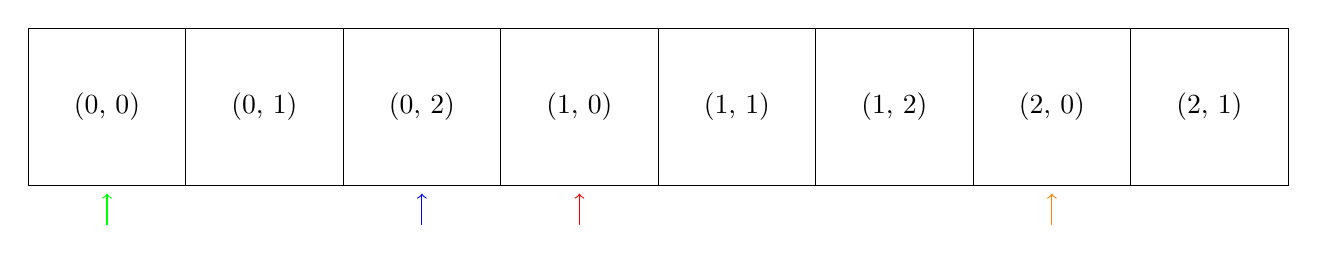
\begin{tikzpicture}
        \draw[step=2cm] (0,0) grid (16,2);

            \node at (1,1) {(0, 0)};
            \node at (3,1) {(0, 1)};
            \node at (5,1) {(0, 2)};
            \node at (7,1) {(1, 0)};
            \node at (9,1) {(1, 1)};
            \node at (11,1) {(1, 2)};
            \node at (13,1) {(2, 0)};
            \node at (15,1) {(2, 1)};        
        \draw[->,red] (7,-0.5) -- (7,-0.1);
        \draw[->,blue] (5,-0.5) -- (5,-0.1);
        \draw[->,green] (1,-0.5) -- (1,-0.1);
        \draw[->,orange] (13,-0.5) -- (13,-0.1);
    \end{tikzpicture}
    \captionof{figure}{Curseurs des employés à placer sur la liste des positions.}
    \label{fig:tableau_positions}
\end{center}

Pour réaliser le déplacement du curseur, nous avons dans un premier temps implémenté une fonction récursive présentée en listing~\ref{lst:deplacer_curseur}.\\

\begin{lstlisting}[style=customstyle]
fonction deplacer_curseur(curseur, i, nb_employes, nb_positions) :
    si (curseur[i] = (nb_positions - (nb_employes - i))) :
        si (i = 0) :
            pour j allant de 0 a nb_employes - 1 :
                curseur[j] <- 0;
            fin pour;
            retourner ; 
        fin si;
        deplacer_curseur(curseur, i - 1, nb_employes, nb_positions);  
        curseur[i] <- curseur[i - 1] + 1; 
    sinon :
        curseur[i] <- curseur[i] + 1;
fin fonction;

\end{lstlisting}
\captionof{lstlisting}{Fonction récursive pour déplacer le curseur}
\label{lst:deplacer_curseur}
\vspace{1cm}
Celle-ci déplace le curseur d'indice \(i\) de la liste (dans notre fonction principale nous n'appelons à déplacer que le dernier curseur).
Pour ce faire, on vérifie si notre indice est à la fin du tableau des positions, si ce n'est pas le cas, on peut le faire avancer de un, sinon nous avançons le curseur précédent de 1 et le replaçons à la suite du précédent. Nous réalisons cela de façon récursive avant de pouvoir déplacer les curseurs précédents en ayant la même logique que pour le dernier.\\ \\
Cette fonction a une complexité en \(O(n)\) où \(n\) est le nombre d'employés à placer.
Cependant, afin de réduire le temps d'exécution de celle-ci, nous avons par la suite réalisé une fonction équivalente itérativement, toujours de complexité \(O(n)\), mais permettant de réduire l'utilisation de la pile et les appels mémoire.

\subsubsection{Comparaison des vecteurs de ressources}
Afin de comparer les différents vecteurs de ressources associés aux listes de positions testées, nous avons réalisé une fonction pour tester si un vecteur était plus grand ou incomparable à un autre.\\
Retournant vrai si le vecteur de ressource \texttt{a} a au moins une ressource supérieure à l'un des vecteurs de ressources parmi la liste de ceux que l'on a décidé de conserver.\\ \\
À l'inverse, si cette fonction renvoie vrai, nous voulons ajouter ce vecteur de ressources à la liste des vecteurs de ressources que l'on conserve. Pour cela, nous vérifions s'il n'existe pas dans cette liste un vecteur inférieur au nouveau (toutes ses composantes sont inférieures). Si c'est le cas, nous le supprimons de la liste en décalant l'ensemble des éléments suivants de -1.\\ \\
Ces problèmes sont résolus en \(O(n \times v)\) où \(n\) est le nombre de ressources à comparer et \(v\) le nombre de vecteurs de ressources à comparer.

\subsubsection{Algorithme global}
Pour résoudre le problème d'optimisation des positions, nous avons finalement réalisé l'algorithme présenté en listing~\ref{lst:algorithme_global}.\\
\begin{lstlisting}[style=customstyle]
positions_libres <- lister_positions_libres'('')';
ressources <- calculer_ressources'('positions_libres')';
candidats_selectionnes <- [];

pour i allant de 0 a nb_employes :
    curseur[i] <- i;
fin pour;

pour i allant de 0 a max_combinations :
    candidat <- creer_candidat'('curseur, positions_libres')';
    deplacer_curseur'('curseur')';
    calculer_ressources_candidat'('candidat, ressources')';
    si '('plus_grand_ou_incomp'('candidat, candidats_selectionnes')'')' :
        ajouter_candidat'('candidats_selectionnes, candidat')';
    fin si;
fin pour;

retourner selectionner_positions_optimales'('candidats_selectionnes')';
\end{lstlisting}
\captionof{lstlisting}{Algorithme global pour l'optimisation des positions}
\label{lst:algorithme_global}
\vspace{0.5cm}
Celui-ci cherche l'ensemble des positions libres du plateau, et pour celles-ci calcule en amont les ressources que l'on peut gagner. Ensuite, pour chaque combinaison de positions possibles, on crée un "candidat" (structure contenant la liste des positions et le vecteur de ressources associé) que l'on compare aux candidats déjà sélectionnés. Pour l'ajouter ou non à la liste des candidats sélectionnés. Enfin, une fonction sélectionne parmi tous les candidats celui qui est le plus optimal par rapport à la configuration du plateau et renvoie ses positions.\\ \\
Un point intéressant à noter pour l'implémentation en \texttt{C} de cet algorithme est lié à la taille du tableau \texttt{candidats\_selectionnes}, celui-ci pourra contenir dans le pire des cas \(\binom{n}{k}\) éléments, ce qui donne rapidement une allocation mémoire beaucoup trop élevée pour être supportée par la pile. Une première solution avait consisté à utiliser une bibliothèque externe calculant la taille de la pile et de nos éléments pour en déduire la taille maximale de notre tableau de façon "dynamique" et renvoyant une erreur si nous tentons d'ajouter plus de candidats à la liste que la taille supportée par l'ordinateur (ce qui était relativement improbable d'arriver au vu du rapport entre la taille de la pile et la quantité moyenne d'éléments stockée à chaque exécution). Or cette méthode pourrait tout de même continuer à générer des erreurs notamment dans le cas où la pile est beaucoup utilisée par une autre partie de notre programme. \\ \\
La méthode la plus simple pour résoudre ce problème a été d'allouer dynamiquement la mémoire en utilisant des \textit{malloc}. Nous aurions aussi pu définir une taille maximale de 100 éléments par exemple et effectuer un premier tri si celle-ci est remplie. Nous n'avons pas mis en place cette méthode pour des raisons de simplicité et de rapidité d'implémentation.

\subsubsection{Complexité de l'algorithme global}
Pour résoudre le problème d'optimisation des positions, l'algorithme parcourt toutes les combinaisons possibles de \(k\) employés (considérons \(k\) fixé à 4), placés sur \(n\) positions, soit \(\binom{n}{4}\) combinaisons. Pour chaque combinaison, il effectue des comparaisons initialement calculée de complexité \(O(n \times v \times \binom{n}{4})\), où \(v\) est dans le pire des cas égal à \(\binom{n}{4}-1\), car on a au maximum un candidat par combinaison.\\
On a donc une complexité totale de \(O(\binom{n}{4}^2)\), puisque chaque candidat est comparé dans le pire des cas avec tous les autres (par simplification nous avons retiré le \(-1\) qui est négligeable).\\ \\
\( \binom{n}{4} = \frac{n(n-1)(n-2)(n-3)}{4!} = n^4\), on a donc \(O(n^4 \times n^4) = O(n^8).\)
La complexité de cet algorithme est plus élevée que celle étudiée dans la section \hyperref[sec:dec]{\uline{Les décisions}} car elle est polynomiale en \( n \). De plus, dans le cas où \( k \) est variable, la complexité sera alors super-exponentielle.\\ \\
Cette nouvelle méthode apporte des décisions plus précises quant au placement des employés, mais augmente significativement la complexité du programme. Bien qu'appelée moins souvent car elle prévoit à l'avance le placement de l'ensemble des employés, elle reste importante et le choix entre ces deux méthodes relève d'un compromis entre précision et rapidité d'exécution.

\subsection*{Biceps, défi sous-jacent}
\addcontentsline{toc}{subsection}{Biceps, défi sous-jacent}
\label{sec:bds}
Ce dernier achievement a pour objectif de mettre en place différentes missions pour gagner de l'or en fin de partie ou pour augmenter le gain de certains bâtiments.
\subsubsection{Missions de fin de partie}
Afin de pimenter le jeu, nous avons réalisé dans \texttt{game.c} une fonction \texttt{goal} qui regarde les bâtiments de l'ensemble des joueurs encore en jeu. Si un joueur :
\begin{itemize}
    \setlength\itemsep{0.01em}
    \item A construit plus de bâtiments qu'il n'a d'employés, il gagne 3 pièces d'or.
    \item A construit plus de bâtiments que les autres joueurs, il gagne 5 pièces d'or.
    \item A construit 2 bâtiments qui produisent du maïs, il gagne 2 pièces d'or.
    \item A construit 3 bâtiments qui forment une composante connexe, il gagne 2 pièces d'or.
\end{itemize}
Nous ne développerons pas ici les fonctions associées à ces objectifs, car elles sont réalisées avec des conditions simples dans des boucles qui parcourent les éléments en question. Leur complexité est donc linéaire.

\subsubsection{Objectifs de gain de bâtiments}
Dans un second temps, nous avons réalisé une mise à jour sur les bâtiments afin de créer des missions associés à chaque bâtiment différent.\\
Ainsi, à l'aide d'un pointeur vers une fonction dans la structure de nos bâtiments, nous avons pu faire en sorte en fin de tour de vérifier certaines conditions associées aux bâtiments et augmenter les ressources qu'ils permettent de gagner selon ces conditions~\cite{renault2024} :
\begin{itemize}
    \setlength\itemsep{0.01em}
    \item \textit{La cathédrale gagne 1 Gold par employé présent sur une de ses positions voisines;}
    \item \textit{Le château gagne 1 Gold par bâtiment présent dans sa composante connexe;}
    \item \textit{La tour de garde gagne 1 Gold par position voisine vide libre;}
\end{itemize}

